
%% bare_conf.tex
%% V1.4b
%% 2015/08/26
%% by Michael Shell
%% See:
%% http://www.michaelshell.org/
%% for current contact information.
%%
%% This is a skeleton file demonstrating the use of IEEEtran.cls
%% (requires IEEEtran.cls version 1.8b or later) with an IEEE
%% conference paper.
%%
%% Support sites:
%% http://www.michaelshell.org/tex/ieeetran/
%% http://www.ctan.org/pkg/ieeetran
%% and
%% http://www.ieee.org/

%%*************************************************************************
%% Legal Notice:
%% This code is offered as-is without any warranty either expressed or
%% implied; without even the implied warranty of MERCHANTABILITY or
%% FITNESS FOR A PARTICULAR PURPOSE! 
%% User assumes all risk.
%% In no event shall the IEEE or any contributor to this code be liable for
%% any damages or losses, including, but not limited to, incidental,
%% consequential, or any other damages, resulting from the use or misuse
%% of any information contained here.
%%
%% All comments are the opinions of their respective authors and are not
%% necessarily endorsed by the IEEE.
%%
%% This work is distributed under the LaTeX Project Public License (LPPL)
%% ( http://www.latex-project.org/ ) version 1.3, and may be freely used,
%% distributed and modified. A copy of the LPPL, version 1.3, is included
%% in the base LaTeX documentation of all distributions of LaTeX released
%% 2003/12/01 or later.
%% Retain all contribution notices and credits.
%% ** Modified files should be clearly indicated as such, including  **
%% ** renaming them and changing author support contact information. **
%%*************************************************************************


% *** Authors should verify (and, if needed, correct) their LaTeX system  ***
% *** with the testflow diagnostic prior to trusting their LaTeX platform ***
% *** with production work. The IEEE's font choices and paper sizes can   ***
% *** trigger bugs that do not appear when using other class files.       ***                          ***
% The testflow support page is at:
% http://www.michaelshell.org/tex/testflow/



\documentclass[conference]{IEEEtran}

\usepackage{graphicx}
\usepackage{amsmath}
\usepackage{amssymb}
\usepackage{gensymb}

\graphicspath{ {C:/Users/Marc/Documents/Uni/van2016} }

\hyphenation{op-tical net-works semi-conduc-tor}


\begin{document}

\title{Application and Verbalization of Fuzzy Cognitive Maps in the Case of Flight Passenger Flows}

\author{\IEEEauthorblockN{Marc Osswald}
\IEEEauthorblockA{Swiss International Air Lines Ltd.\\
Basel, CHE\\
Email: marc.osswald@swiss.com}
\and
\IEEEauthorblockN{Marcel Wehrle}
\IEEEauthorblockA{University of Fribourg\\
Fribourg, CHE\\
Email: marcel.wehrle@unifr.ch}
\and
\IEEEauthorblockN{Edy Portmann}
\IEEEauthorblockA{University of Bern\\
Bern, CHE\\
Email: edy.portmann@iwi.unibe.ch}}

\maketitle

\begin{abstract}
This paper seeks to turn the mathematical output of a Fuzzy Cognitive Map (short:~FCM) into natural language sentences with the aid of the Restriction Centered Theory (short:~RCT). The concept of a FCM, a choice of subsequent simulation runs and learning algorithms are presented, evaluated and discussed. The main elements and ideas of the RCT are outlined, and afterwards, these two main topics are linked.\\
The feasibility of the thesis will be emphasized with a use case, where an airline's connecting passenger flows are analyzed. It includes the transformation and import of raw data into a graph database, the creation of statements made in natural language about the FCM's content and the verification of these statements by an expert of the data-owning company.\\
Keywords: Fuzzy Cognitive Map, Restriction Centered Theory, Verbalization, Natural Language, Fuzziness, Graph Database
\end{abstract}

\IEEEpeerreviewmaketitle

\section{Introduction}
Dealing with language is simple and complicated at the same time. There is a set of rules stating how words have to be arranged in order to build grammatically correct sentences. By learning and following the rules, one is able to speak the language correctly -- in terms of grammar. The big challenge of using a language is to find exactly those words that express what someone wants to communicate to its counterpart. But it is not guaranteed yet that the listener will interpret these words in the same way as the speaker does. Rapaport \cite{Rapaport2003} says that communication is a negotiation of meanings. If two people do not have a common understanding of the concept behind a word, they will experience a misunderstanding.\\
For computers, the meaning of a sentence cannot be recognized unless he is taught by a human to do so. There are many ways to convert complex information into bits and bytes. But information are supposed to flow also in the other direction. Computers need to be able to decide themselves, which part of the information is relevant and which one is not. And there must be a way to communicate their findings to a human not only in digits, but in complete sentences.\\
These sentences should be filled with meaningful words. Statements like "In the past three years, the maximum temperature on Easter Sunday was (5.1\degree C, 6.2\degree C, 2.3\degree C)" are then replaced by "In the past three years, Easter Sunday was always a cold day". At the same time, the problem of subjectivity raises. If someone thinks that every temperature above 0\degree C does not deserve the name "cold", then he might be misled by the information. Even worse, if someone has its limit at 5\degree C, then even the word "always" is not correct anymore.\\
This kind of difference in interpretation of words is a big problem for computers. But there is a way to avoid this strict allocation of content to a concept: Fuzzy computation. It allows that absolute values like temperatures belong not only to a single, but to different concepts.\\
This paper seeks to find a way to shape cognitive maps out of keywords, to enrich them with fuzziness with the aid of large data amounts, to learn from these fuzzy cognitive maps (short: FCM) by applying learning algorithms. And, as a last step, to phrase the lessons learned into complete and meaningful sentences.\\
In order to achieve this, the following questions are to be answered:
\begin{itemize}
\item How does a FCM work?
\item What is the Restriction Centered Theory?
\item Can the Restriction Centered Theory be applied to Fuzzy Cognitive Maps?
\end{itemize}

\section{Theory of FCM and RCT}
\subsection{Fuzzy Cognitive Maps}
The widely known mind map is at the roots of the FCM. A mind map starts with a central term or concept. Other terms that are associated with this initial term, are written around the first one and linked with graphs to each other. These associated terms may be used as central nodes as well so that in the end a tree structure is formed.\\
It is obvious that most of the concepts cannot be described in tree structures only. The road networks of some nations with a centralistic structure, such as France, remind to this way of conceptualization. Many roads are leading to Paris, the capital. But clearly, there is the need of links between smaller towns in case that someone who wants to get from Lyon to Marseille is not forced to make a detour via Paris.\\
These direct interconnections expand the tree structure of the mind map by an important element. Links between any elements of the map can be represented this way. As a consequence there is not a simple tree structure anymore, but there can occur cycles. This is much closer to reality and a huge step forward towards the cognitive map.\\
It is not necessarily roads but any kind of precise or abstract concepts that can be interconnected in cognitive maps. Hereby, the concepts are represented by nodes, the interconnections by directed graphs. Additionally the edges are used for representing the information of how a concept influences another. This information is reduced to a plus or minus, meaning that a concept exerts a positive or a negative influence to its counterpart.\\
The last step towards the FCM is now the introduction of edge weights in the interval between -1 and 1. This makes it possible to give a statement about how much a concept influences another.\\
According to Stach et al. \cite{stach2005} a FCM can be developed either manually or computationally. A good illustration is done by Montazemi and Conrath \cite{montazemi1986}, who propose such a cognitive map investigating the influence factors of population growth and the role of sanitation facilities in fighting diseases in the city. It has been constructed for a fictive Director of Public Health seeking for a cause why the number of diseases increased despite the improvement of the sanitation facilities in his city.
\begin{figure}[h]
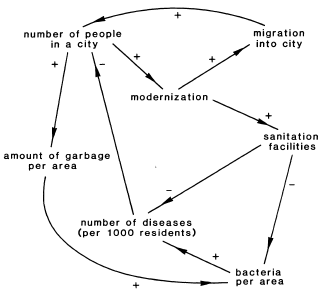
\includegraphics{CognitiveMap.png}
\caption{Cognitive Map for Director of Public Health}
\label{fig:cm}
\end{figure}

\subsubsection{Formal Definition of FCM}
The following formal definition has been done by Stach et al. \cite{stach2005}. It provides a possibility to dynamically calculate a FCM with iterative steps. Let \begin{math} \mathbb{R} \end{math} be the set of real numbers, while \begin{math} \mathbb{N} \end{math} denotes the set of natural numbers. \begin{math} K = [-1,1] \end{math} and \begin{math} L = [0,1] \end{math}. A Fuzzy Cognitive Map \begin{math} F = [-1,1] \end{math} is a 4-tuple \begin{math} (N,E,C,f) \end{math}, where
\begin{enumerate}
\item \begin{math} N = {N_{1},N_{2},...,N_{n}} \end{math} is the set of n concepts forming the nodes of a graph.
\item \begin{math} E: (N_{i},N_{j}) \rightarrow e_{ij} \end{math} is a function of \begin{math} N \times N \end{math} to \begin{math} K \end{math} associating \begin{math} e_{ij} \end{math} equal to zero if \begin{math} i = j \end{math}. Thus \begin{math} E(N \times N) = (e_{ij}) \in K^{n \times n} \end{math} is a connection matrix.
\item \begin{math} C: N_{i} \rightarrow C_{i} \end{math} is a function that at each concept \begin{math} N_{i} \end{math} associates the sequence of its activation degrees such as for \begin{math} t \in \mathbb{N}, C_{i}(t) \in L \end{math} given its activation degree at the moment \begin{math} t \end{math}. \begin{math} C(0) \in L^{n} \end{math} indicates the initial vector and specifies initial values of all concept nodes and \begin{math} C(t) \in L^{n} \end{math} is a state vector at certain iteration \begin{math} t \end{math}.
\item \begin{math} f: \mathbb{R} \rightarrow L \end{math} is a transformation function, which includes recurring relationship on \begin{math} t \geq 0 \end{math} between \begin{math} C(t+1) \end{math} and \begin{math} C(t) \end{math}.
\end{enumerate}
A simulation run on a FCM starts with a scenario which is expressed in an initial vector. This vector is included in the functional model. The result of the calculation step is a new vector, the so-called state vector. The relationship between the initial vector and the iteration result is a cause-effect statement.\\
When iterating the FCM for several times, it is possible that a pattern can occur. The sequence of the state vectors is then repeating. If the state vector does not change anymore, the FCM is in a steady state. On the other hand it is also possible that with every iteration a new state vector is produced. This kind of FCM is called chaotic.\\
The functional model described by Stach et al. \cite{stach2005} is as follows:\\
\begin{equation}
\forall i \in \{1,...,n\},C_{i}(t+1) = f  \bigg(\sum_{i=1 \atop i \neq j}^{n} e_{ji}C_{j}(t)\bigg)
\end{equation}
In this way, the initial vector is being multiplied with the vector of corresponding edge weights. Since these weights are supposed to be fuzzy, a transformation function is used to stick to a certain range defined at the beginning. There are many different ways to normalize the values, the most common ones according to Stach et al. \cite{stach2005} are the following:
\begin{itemize}
\item bivalent: \begin{math} f(x) = \begin{cases} 
0 & \text{if } x \leq 0\\ 
1 & \text{if } x > 0
\end{cases} \end{math}
\item trivalent: \begin{math} f(x) = \begin{cases}
-1 & \text{if } x \leq -0.5\\
0 & \text{if } -0.5 < x < 0.5\\
1 & \text{if } x \geq 0.5
\end{cases} \end{math}
\item logistic: \begin{math} f(x) = \frac{1}{1+e^{-cx}}, c \in \mathbb{R} \end{math}
\end{itemize}
In order to interpret a FCM at a first glance, several key indicators can be used. According to \"Ozesmi and \"Ozesmi \cite{ozesmi2004}, a node can be classified into three types: transmitter, receiver and ordinary. The determination is done based on two key figures, outdegree and indegree. The outdegree \begin{math} od_{i} \end{math} of a node \begin{math} N_{i} \end{math} is the sum of its outgoing absolute edge weights, while the indegree \begin{math} id_{i} \end{math} of node \begin{math} N_{i} \end{math} sums the absolute weights of all incoming edges.\\
\begin{equation}
od_{i} = \sum_{j=1}^{n}|e_{ij}|
\end{equation}
\begin{equation}
id_{i} = \sum_{j=1}^{n}|e_{ji}|
\end{equation}
If a node has a positive outdegree and zero indegree, it is a transmitter node. If it has zero outdegree and positive indegree, it is a receiver node. If both of the degrees are positive, it is an ordinary node.\\
The relevance of a node within the FCM can be expressed with the centrality \begin{math}td_{i} \end{math} which is simply the sum of outdegree and indegree. The higher this number, the higher the influence on the FCM. Finally, the connectivity of the whole FCM can be measured with the density \begin{math} d \end{math}, which is the ratio of existing to all possible connections.\\

\subsubsection{Learning Algorithms for FCM}
It is often problematic to argue about the edge weights of a FCM. Usually they are determined by human interaction. Depending on the field of research this process is heavily subjective. An approach to solve this problem are learning algorithms.\\
There are many different ways to learn by modifying edge weights. A first departure is done by Dickerson and Kosko~\cite{dickerson1993}, who proposed Differential Hebbian Learning (DHL) law to be applied to FCM:
\begin{equation}
\dot{e}_{ij} = -e_{ij} + \dot{C}_{i}\dot{C}_{j}
\end{equation}
In this equation, \begin{math} \dot{e}_{ij} \end{math} stands for the change of weight between nodes \begin{math}N_{i} \end{math} and \begin{math}N_{j} \end{math}, \begin{math} e_{ij} \end{math} is the current weight and \begin{math} \dot{C}_{i} \end{math} and \begin{math} \dot{C}_{j} \end{math} are changes of the activation degree of nodes \begin{math} N_{i} \end{math} and \begin{math} N_{j} \end{math}. Expressed in a discrete way, the update equation is defined as:
\begin{equation}
e_{ij}(t+1)= \begin{cases}
e_{ij}(t) + c_{t} [ \Delta C_{i} \Delta C_{j} - e_{ij}(t)] & \text{if } \Delta C_{i} \neq 0\\
e_{ij}(t) & \text{if } \Delta C_{i} = 0
\end{cases}
\end{equation}
The concepts are moving in the same direction if \begin{math} \Delta C_{i} \end{math} and \begin{math} C_{j} \end{math} are both either positive or negative. In these cases the edge weights would move towards the minimum (-1) or maximum (1) weight. If concepts are moving in different directions, the algebraic signs of \begin{math} C_{i} \end{math} and \begin{math} C_{j} \end{math} are not equal. Then, edge weights would move towards zero, which is in the middle of the value range.\\
There exist several extensions of this DHL method, for example the Balanced Differential Algorithm (BDA), the Nonlinear Hebbian Learning (NHL) or the Active Hebbian Learning (AHL). The BDA was introduced by Huerga \cite{huerga2002} who criticized the fact that DHL only considers state changes of the outgoing node. In his algorithm every node that shows the same behavior is included. One of the most important drawbacks is that the algorithm is only applicable to a bivalent value range.\\
The NHL, presented by Papageorgiou, Stylios and Groumpos \cite{papageorgiou2003}, considers only updates of edge weights that are initially chosen. This selection is done by a human interaction which is the main disadvantage of this algorithm.\\
Another proposal made by Papageorgiou, Stylios and Groumpos \cite{papageorgiou2004} is the AHL. Here the sequence of activated nodes as well as one or multiple nodes where the main focus is put on, are initially defined by the creators of the FCM. These nodes are decisive in determining whether the algorithm stops or not. The main problem is again the necessity for human interaction, although it is only needed at the beginning of the process.

\subsection{Restriction Centered Theory}
With a word, a human can express fuzziness in a much simpler way than using complex probabilistic models. The challenge is to transform these words into a computable form. In brief, this is what RCT is seeking for.\\
\subsubsection{General Idea of the RCT}
If an answer to the question "How true is X?" is expressed with an interval, the range of the value is a numerical value between 0 and 1 (or likewise the interval is defined). The same is valid for a set with predefined values or a probability distribution. Each of these concepts has a homogeneous range. A word can be used in two different ranges, that is, in two different contexts. And, even worse, according to the context it is used in, the same word can have different meanings.\\
The central concept of the RCT is the restriction. It can be implemented in a more general way than an interval, a set or a probability distribution. The range of a restriction is a melting pot with all the concepts mentioned, it can take any value you can think of. To recognize the size of this range, here an example: If a human is asked a question like "How tall is Steve?", his answers might be "Steve is 1.85m tall", "Steve is 6 feet 1 inch tall", "Steve is quite tall", "Steve is taller than Angelica", "Steve is not as tall as Michael is", "Steve is between 5 and 10 cm taller than me" and so on.\\
The first two statements do not bear any room for ambiguity, the last four of these restrictions are theses, in Zadeh \cite{zadeh2013} called propositions. They are drawn from natural language and do usually contain a fuzzy component such as a predicate (small, strong, slow), a quantifier (lots, little, more) and/or a probability (likely, unlikely). A distinction between zero-order and first-order fuzzy propositions is made, where the former does only contain a fuzzy predicate, while the latter contains any one or more of the components mentioned.\\
A computer asking how tall Steve is, can interpret only the first two answers, unless it is able to turn the proposition into a computable form. With the RCT, this turns out to be feasible.\\
To represent a proposition made in natural language in a mathematical form, the Meaning Postulate (short: MP) is used:
\begin{equation} \label{eq:mp}
p \rightarrow X isr R
\end{equation}
In this equation, \begin{math} p \end{math} is the proposition that contains a variable to be restricted, \begin{math} X \end{math}, a restricting relation, \begin{math} R \end{math}, and the type of the restricting relation, \begin{math} r \end{math}. The better \begin{math} X \end{math}, \begin{math} R \end{math} and \begin{math} r \end{math} are mathematically defined, the better a restriction can be computed. Computations with restrictions look as pointed out in this example with fictive numbers: "One out of about 100'000 people are affected by the genetic disorder called maple syrup urine disease. In Switzerland, some 20 people are affected by this disease. What is the population of Switzerland?" These two restrictions implicate that Switzerland has only two million inhabitants. Humans are used to deal with this kind of fuzzy reasoning. RCT offers the approach to solve these problems computationally.\\
A second important element of the RCT is the Canonical Form (short: CF). Basically, \begin{math} CF(p) \end{math} is the right-hand side part of Equation~\ref{eq:mp}, assigning the correct restriction type to the proposition.\\
The last element to be mentioned is the Truth Postulate (short: TP). It measures the truth degree of a MP and is closely linked to the preciseness of the proposition. The truth degree can be expressed either numeric, called first-order truth value, or in natural language, which is a second-order truth value.
\subsubsection{Restrictions}
A restriction is called singular if the type of the restricting relation, \begin{math} R \end{math}, is a singleton, e.g. \begin{math} X=5 \end{math}. It’s called nonsingular if \begin{math} R \end{math} is not a singleton. The restricted variable may be \begin{math} X \end{math} or a function of \begin{math} X \end{math}. In the first case, the restriction is called direct, otherwise indirect. A restriction can be differentiated into types. The three most important types are the possibilistic restriction, the probabilistic restriction and the Z-restriction which is a combination of the two former types.\\
In the possibilistic restriction, \begin{math} R \end{math} is a fuzzy set, \begin{math} A \end{math}, where \begin{math} X \end{math} belongs to. The affiliation of \begin{math} X \end{math} to \begin{math} A \end{math} is evaluated with the membership function, \begin{math} \mu_{A} \end{math} , of a possibility distribution. The same is valid for fuzzy relations where two variables are compared.\\
With the probabilistic restriction, a statement about the certainty of a proposition can be made. This is evaluated with a density function of \begin{math} X \end{math}. Applied to statements with natural language this means that the certainty of "usually" is higher than the one of "sometimes". It is very rare that probabilistic restrictions occur exclusively in natural language, they are rather to find in combination with a possibilistic proposition. This combination is called a Z-restriction. It incorporates natural language propositions, such as for example "Maybe Person A is young", where "young" is possibilistic and "maybe" probabilistic.\\
The notation of the CF is differing depending on the type of restriction. A possibilistic restriction is denoted as \begin{math} X is A \end{math}, where \begin{math} A \end{math} is the fuzzy set or relation. A probabilistic restriction is shown as \begin{math} X isp p \end{math}, where the first \begin{math} p \end{math} is the probability density function (not to be mistaken with the second \begin{math} p \end{math} for proposition in the MP). A Z-restriction is indicated as \begin{math} X iz Z \end{math}, where \begin{math} Z \end{math} is the combination of possibilistic and probabilistic restrictions defined as \begin{math} Z: Prob(X is A) is B \end{math}.\\
In most of the cases, the restriction is formulated in natural language. The process of transforming the linguistic input into a computable form, is called precisiation. To achieve this, a so-called explanatory database (short: ED) is used, which is a collection of relations containing the data source to precisiate the variables \begin{math} X \end{math} and \begin{math} R \end{math}, or to compute the truth value of \begin{math} p \end{math}. If the variables are precisiated, they are denoted by \begin{math} X^{*} \end{math}, \begin{math} R^{*} \end{math} and \begin{math}p^{*} \end{math}. So, \begin{math} X^{*}=f(ED) \end{math} and \begin{math} R^{*}=g(ED) \end{math}. The numerical truth value of \begin{math} p \end{math}, \begin{math}nt_{p} \end{math}, can be expressed as \begin{math} nt_{p}=tr(ED) \end{math}, where \begin{math} tr \end{math} is referred to as the truth function.

\section{Architecture and Framework}
It is now shown how natural language can be turned into a computable input. If there exists a FCM with nodes, edges and their respective weights, the computable input is available, but cannot be interpreted by an unexperienced person. So how is it possible to convert the mathematical input of a FCM into natural language with the aid of the RCT?\\
First of all, it has to be made clear, how the RCT can make use of a FCM: The FCM is usually built based on experiences, whether the experts' thoughts and observations or another big amount of data. So, the FCM has to serve as the ED for the RCT, since it provides the data that is used to precisiate variables.
In order to build a sentence, grammatically, at least a subject and a predicate is required. As a subject, a certain node of the FCM can be utilized, regardless of any context. The predicate has to be defined by the user, depending on the statement that he wants to make. After all, this is not very informative yet.
Therefore, two further elements have to be added to a standard sentence: An object, where another node can be placed, as well as a descriptive word like an adjective or adverb. It is thinkable that the edge weight can be used for this purpose, since it gives an idea about the strength of a relationship between subject and object. Depending on the weight, a certain word is chosen to describe the content.
Here, the RCT comes into play. The choice of words is similar to a possibilistic restriction. Each word has a different membership function. The totality of word options should cover the whole range of edge weights. The membership degree of each eligible word has then to be evaluated and the maximum among them is to be chosen. If there are two or more words with the same membership degree, it has to be assumed that these words can be used similarly.
A different nature of statements can also be made based on key figures such as the outdegree or the centrality of a node. Also, the state of a node at a certain moment during a simulation bears instructive information.
The nature of statements is strongly depending on the content of the FCM. This context-dependency is what makes it very difficult to define, for example, clear sets of words that can be used for any purpose. In the following chapter, a use case will be defined to get an idea of what is possible and what is not.

\section{Use Case Swiss: FCM model to describe flight passenger flows}
The following use case will investigate on the passenger flows of an airline. A FCM will be constructed based on connecting passengers, a simulation will be ran and then, the result shall be interpreted by a tool called interpretation engine, or engine, converting the output into natural language statements.\\
The data for this use case was provided by Swiss (airline code: LX). It contains 1'371'280 passenger records from January 2013, all these passengers travelled with one or more flights operated by LX. Every record contains the following information: Origin and destination of the traveler's journey (in separate fields), departure and arrival of the segment, flight number (operator and number in separate fields) and the document number.\\

\subsection{Design of the FCM}
When designing a new FCM, the specifications of the nodes, the graphs and the properties have to be determined before importing the data. The nodes are depicted as routes. Hence, a connecting passenger from Los Angeles through Zurich to Paris would be depicted as a link from the node ZRH-LAX to the node ZRH-CDG, as shown in Figure \ref{fig:noderoute}. The intermediate airport is mentioned twice in the node. If an airline has more than only one main hub, it is important to be able to distinguish the routes between the hubs. With the route node specification, this is assured.
\begin{figure}[h]
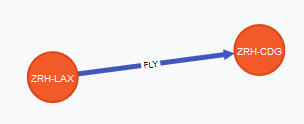
\includegraphics{noderoute.png}
\caption{Specification of FCM Nodes as Routes}
\label{fig:noderoute}
\end{figure}
A problem to be solved are people who connect from another airline to Swiss flights. In any case it is necessary to identify these passengers as external connectors, since their share on certain routes is substantial for the airline. If they are not identified they are just counted as regular, non-connection passengers, which is unacceptable. Therefore, they need to be aggregated in a specific node. Hence, any route not being in the network is eliminated and the passengers can be identified on the route.\\
Following these argumentations, a node will be created for every route being in the network of Swiss. Its name will be composed by the two airports, first the hub and then the destination. If no hub is involved, then the airports will be referred to in alphabetical order. A separate node for all routes outside of Swiss' network will be created. Its name is OA, which stands for "Other Airline".\\
The specification of the graphs is straightforward: A graph has to be set if a passenger flies on two routes within the same journey. The graph points to the direction of travel.\\
The remaining thing to be specified are the properties of the FCM's elements. Nodes hold the information about their name, that is, the route. A description is added, where the route is mentioned in plain text. And, finally, the total number of passengers traveling on this route is provided. It includes all passengers, be it connecting or not. Graphs hold the information about the route where a passengers comes from and the one it is connecting to. Also, the number of passengers on the graph as well as the ratio between the number of connectors and the total number of passengers on the original route is provided.\\

\subsection{Query Engine}
In order to interpret the FCM, a query engine has to be defined that generates sentences in natural language. These statements are delivering a deeper insight into the FCM and allow a simpler interpretation of the data. For the present use case, two different issues are considered: 
\begin{itemize}
\item The frequency of connecting passengers between two specific routes in a directed sense
\item The frequency of connecting passengers on a specific route to any other.
\end{itemize}
A third issue, the frequency of connecting passengers to a specific route from any other one could not be analyzed with the present data.\\
It is to mention that the frequency of connecting passengers from one route to another in relation to the total number of passengers on the first route, is very low. There are 4'050 different connections between two routes, the median is at 0.2\%, and the 90\%-percentile is at 1.1\%. This means that most of the connections have a very low share, which is why it is important to have an accurate distinction on low shares, whereas the shares above 20\% can be described with very few different words.\\
The frequency of connection passengers from one route to any other is, of course, higher than the first one. Here, the median is at 25\% and the 90\%-percentile is at 43.4\%. Therefore, the range between 20\% and 100\% of connections shall be described with five different adjectives. The remaining range between 0\% and 20\% will be covered with nine different adjectives.\\
All of the adjectives are supposed to express the frequency of a connection and are herewith ordered according to the frequency: Never, seldom, rarely, occasionally, infrequently, sometimes, frequently, often, regularly, normally, usually, generally, hardly ever, and always. Each of these words has got a membership function that defines the word's degree of truth in relation to the share of connecting passengers. When building the sentence, the word with the maximum membership degree is chosen, since it matches best the meaning that needs to be given to the sentence. Words with equal degrees can be used synonymously.\\
The frame of the sentences has to be defined for both issues that are considered. For the first issue, passengers that connect between two specific routes in a directed sense, the frame will be: \newline \emph{"Passengers travelling from (a) to (b) [c] connect to (d)."} \newline In this sentence, \emph{(a)} is the starting point of the journey which is normally the ending point of the route node, since the hub is always mentioned in first position. Then, \emph{(b)} is the hub, in which the passengers connect to the next flight. \emph{[c]} signifies the adjective, describing the frequency of connections and, finally, \emph{(d)} represents the ending point of the connection.\\
The second issue that is considered in the use case, describes the frequency of connecting passengers from a specific route to any other route. Here, the frame will be: \newline \emph{"Passengers travelling on the route (a) [b] connect to another flight."} \newline Here, only the route \emph{(a)} and the describing word \emph{[b]} are used. Thus, it is a more general statement about connecting passengers, but nevertheless, the importance for analysis is at least as big as for the first issue.

\subsection{Verbalization of the FCM}
After having defined and created the FCM, some specific connecting combinations are investigated. The first issue is the connection from New York (JFK) via Zurich (ZRH) to Tel Aviv (TLV). The rate of passengers connecting from ZRH-JFK to ZRH-TLV is 0.0298. Based on this value, the truth value is now calculated for every adjective. There are two words having a maximum truth value of 1, that is, rarely and occasionally. These words can be used synonymously, which means that one word can be picked randomly. The sentence to be built would then be: \newline \emph{"Passengers travelling from New York JFK to Zurich \textbf{occasionally} connect to Tel Aviv."} \newline Some other ten sentences are built in the same way. The choice of connections should cover the whole variety of long and short haul combinations, as well as journeys through all the three hubs. All the generated sentences are listed below:
\begin{enumerate}
\item Passengers travelling from Dar es Salaam to Zurich often connect to London Heathrow.
\item Passengers travelling from Palma de Mallorca to Geneva frequently connect to Zurich.
\item Passengers travelling with Other Airlines never connect to the route Zurich-Birmingham.
\item Passengers travelling from Barcelona to Zurich never connect to Tokyo.
\item Passengers travelling from Tokyo to Zurich infrequently connect to Barcelona.
\item Passengers travelling from Barcelona to Basel seldom connect to Hamburg.
\item Passengers travelling from Mumbai to Zurich rarely connect to Manchester.
\item Passengers travelling on the route Zurich-Lyon usually connect another flight.
\item Passengers travelling on the route Geneva-London Heathrow occasionally connect to another flight.
\item Passengers travelling on the route Zurich-London Heathrow frequently connect to another flight.
\end{enumerate}

\section{Lessons learned}
There were three main points in the user's feedback that need to be improved:
\begin{itemize}
\item The adjective "never" should be replaced by "do not"
\item The number of adjectives should be reduced
\item The adjective "usually" should be replaced by a different, unspecified word
\end{itemize}
It is true that the word "never" implies a certain finality, saying that passengers do not connect neither now nor in future between two routes. Therefore it makes sense to replace it by a word such as "do not" which rather makes a statement about the content and does not imply anything for future periods.\\
In order to simplify business decisions it makes sense to reduce the number of adjectives. Each word would then cause a specific decision to be made. However, the sense of the tool is supposed to depict a big spectrum of adjectives, and hence, the tool can be used for a pre-analysis pointing out fields where deeper analysis is necessary. The business decisions should then be taken based on these further analyses.\\
In a user's perception, the word "usually" is based on a standard that is either fulfilled or not. Since this standard is varying on every route and possibly even in every month, he disadvises the usage of the adjective. The shares that are used for choosing the word are based on the share of connecting passengers on the original route. Hence, the rating basis is varying on every route by definition. But, it is true that the seasonal factor, which has a very high importance in airline industry, is not considered in the tool. Doing so would imply a heavily higher data load and a time related dimension, which was not acceptable for the present use case.

\section{Conclusion}
FCM are used in many different fields of application: Medicine \cite{georgopoulos2003}, Ecology \cite{ozesmi2004}, Economy \cite{carvalho2004}, IT Project Management \cite{rodriguez2007} and many more. The interpretation of the underlying FCM was preferentially done with If-Then sentences, where a premise leads to a specific result.\\
This kind of interpretation contradicts the concept of fuzziness fundamentally, even though it is possible to formulate the premise as "If something is true to 0.2, then...". But the basic idea of having concepts and measuring the degree of membership in a fuzzy way is complex, because every fuzzy membership has to be expressed in many different If-Then clauses. With the possibilistic distribution, the RCT provides an instrument that eases the allocation of fuzzy membership degrees to concepts.\\
With the chosen approach of turning FCM output into natural language with the aid of the RCT, the interpretation of the FCM is left to the experts who build the FCM. They are in lead to define the sentence framework, to precisiate the set of words that is used and to specify the associated membership functions. This bares on one hand the chance that the content is made understandable to a bigger community, on the other hand there is the risk, that some information are manipulated or withheld, be it by mistake or even on purpose.\\
In his paper, Hagiwara \cite{hagiwara1992} points out three major improvement fields of the common FCM: 
\begin{itemize}
\item The proportionality of a relationship between two concepts
\item The lack of time delays
\item The impossibility of representing multiple causality. 
\end{itemize}
Especially the first point is interesting when trying to depict customer behavior in relation to the price, which is usually not linear but elastic. It also shows that the full potential of this approach is not yet exploited by far.\\
Even though graph databases are simple to build and handle, there are only few people using it in daily purpose. It will be interesting to observe, if and how this behavior will evolve. The introduction of a time dimension on the FCM is also to be investigated. This is basically a problem of data size, which is even intensified when combining it with the learning algorithms.\\
On the RCT side the translation of results from the automated pattern recognition into natural language is a field, where many questions are not yet answered, especially in terms of granularity. This would make it possible to evaluate a FCM on an aggregated level and then to infer statements about more detailed parts of the FCM.\\
When reading these perspectives, one has always to keep in mind, that a FCM -- like every model -- is an abstraction of the real world. The goal of an abstraction is to create a simplified picture of complex relations. Many of the above-mentioned ideas do not imply any reduction of complexity when modeling the data with nowadays' technology. Nevertheless, this should be understood as an inspiration and motivation for tomorrow's ambitions.

\section*{Acknowledgment}
The authors would like to thank Mr. Edi Wolfensberger, former Head of Channel Management at Swiss International Air Lines Ltd., who checked the verbalized output of the FCM and gave precious feedback from a user's perspective.

\bibliographystyle{IEEEtran}
\bibliography{fuzzieee2016}

\end{document}


